\chapter{Электричество и магнетизм как единое релятивистское поле}

Мы изучили, как заданное электромагнитное поле приводит в движение заряженную частицу. Незавершенная половина задачи — само поле: как эволюционируют электрическое и магнитное поля и как заряд и ток служат их источниками. На эти вопросы отвечают уравнения Максвелла. Однако прежде чем записывать их, полезно сначала восстановить физическую загадку, из-за которой их релятивистская структура стала неизбежной.

Это намеренное отступление от формализма. Принцип действия еще вернется, но не сейчас. Смысл того, чтобы начать с другого места, состоит в том, чтобы увидеть, почему электрическое и магнитное поля должны быть частями одного объекта, прежде чем выводить их динамику из действия.

\section{Загадка в первом абзаце Эйнштейна}

Во время визита в Бельгию обсуждение ранних Сольвеевских конференций вернуло нас к статье Эйнштейна 1905 года, \emph{Об электродинамике движущихся тел}. В ее первом абзаце с поразительной лаконичностью сформулирована мотивация. Одно и то же электромагнитное явление получает два на вид разных объяснения в двух инерциальных системах отсчета. Один наблюдатель называет эффект магнитным, другой — электрическим. Наблюдаемое движение совпадает, так что эти два описания не могут представлять собой два разных физических содержания.

Теперь эту статью можно читать на уровне, достигнутом в этом курсе. Даже если не разбирать каждое вычисление, начальный абзац стоит прочитать, потому что он ставит правильный вопрос прежде, чем вводить ответ: как могут меняться электрическое и магнитное описания, если физическое событие не меняется?

\subsection{Заряд, магнит и два описания}

Возьмем магнитное поле, направленное вдоль \(y\), и заряд, движущийся вдоль оси \(x\). В лабораторной системе отсчета электрическое поле равно нулю, так что сила является магнитной:
\begin{equation}
\mathbf F=q\,\mathbf v\times\mathbf B.
\end{equation}
Она направлена в оставшемся поперечном направлении. Быстрый рисунок осей на доске в лекции не предназначен для того, чтобы фиксировать каждый знак по правилу правой руки; важны следующие факты: сила перпендикулярна и \(\mathbf v\), и \(\mathbf B\), а при изменении знака заряда знак силы меняется на противоположный.

\begin{classroomqa}
\audiencequestion{Сила на рисунке направлена вверх или вниз?}
\lecturerresponse{Это зависит от знака заряда. Как только ориентация осей и знак \(q\) зафиксированы, правило правой руки определяет направление. Для настоящего аргумента важно лишь наличие поперечной силы. \lecturetimestamp{00:07:13}}
\end{classroomqa}

Эйнштейн рассматривал провод, а не изолированную частицу. Атомы образуют приблизительно неподвижную решетку, а подвижные носители заряда движутся сквозь нее. В начале XX века ток в проводе было также намного легче наблюдать, чем траекторию отдельной свободной заряженной частицы. Здесь это различие несущественно: движущийся носитель в магнитном поле испытывает ту же силу Лоренца.

\begin{figure}[H]
\centering
\includegraphics[width=\linewidth]{lecture_08_figure_01.png}
\caption{Движущийся заряд, поперечное магнитное поле и геометрия магнита, используемые для переформулировки электродинамической загадки Эйнштейна.}
\par\smallskip
\textit{Кадр лекции: 00:07:00.}
\end{figure}

Теперь оставим провод, или пробный заряд, неподвижным и будем двигать вместо него магнит. Меняющаяся магнитная конфигурация создает электродвижущую силу, которая в локальном описании является электрическим полем. Это электрическое поле толкает покоящийся заряд в том же поперечном направлении. Таким образом, два описания таковы
\begin{align}
\text{moving charge, fixed magnet:}\quad&
q\,\mathbf v\times\mathbf B,
\\
\text{fixed charge, moving magnet:}\quad&
q\,\mathbf E'.
\end{align}
Относительное движение одно и то же. Поэтому теория относительности должна объяснить, как поле, являющееся чисто магнитным в одной системе отсчета, приобретает электрическую компоненту в другой.

Электричество и магнетизм — не отдельные субстанции. Это зависящие от системы отсчета части одного релятивистского поля. У Эйнштейна еще не было современной записи через тензор поля, и в этом абзаце он не называл требуемые изменения системы отсчета преобразованиями Лоренца. Тем не менее вопрос о преобразовании уже присутствует здесь в полном объеме.

\section{Тензор электромагнитного поля}

Объектом, который может объединять электрические и магнитные данные, является антисимметричный тензор
\begin{equation}
F_{\mu\nu}
=
\partial_\mu A_\nu-\partial_\nu A_\mu.
\label{eq:field-tensor-definition}
\end{equation}
Греческие индексы пробегают значения \(0,1,2,3\), причем \(x^0=t\); латинские индексы пробегают три пространственных значения. Антисимметрия
\begin{equation}
F_{\mu\nu}=-F_{\nu\mu},
\end{equation}
обращает диагональные элементы в нуль и оставляет 6 независимых компонент. Эти 6 — в точности 3 компоненты \(\mathbf E\) и 3 компоненты \(\mathbf B\).

При метрике с преимущественно положительными знаками
\begin{equation}
\eta_{\mu\nu}=\operatorname{diag}(-1,1,1,1),
\end{equation}
и соглашении, унаследованном от действия заряженной частицы в предыдущей лекции, определим
\begin{align}
E_m&=F_{0m}
=\partial_0A_m-\partial_mA_0,
\label{eq:e-from-a}
\\
B_i&=(\boldsymbol\nabla\times\mathbf A)_i.
\label{eq:b-from-a}
\end{align}
В лекции при записи первой строки исправляется пространственный индекс. Правильное соотношение приведено выше: свободный пространственный индекс должен совпадать в обеих частях.

\begin{figure}[H]
\centering
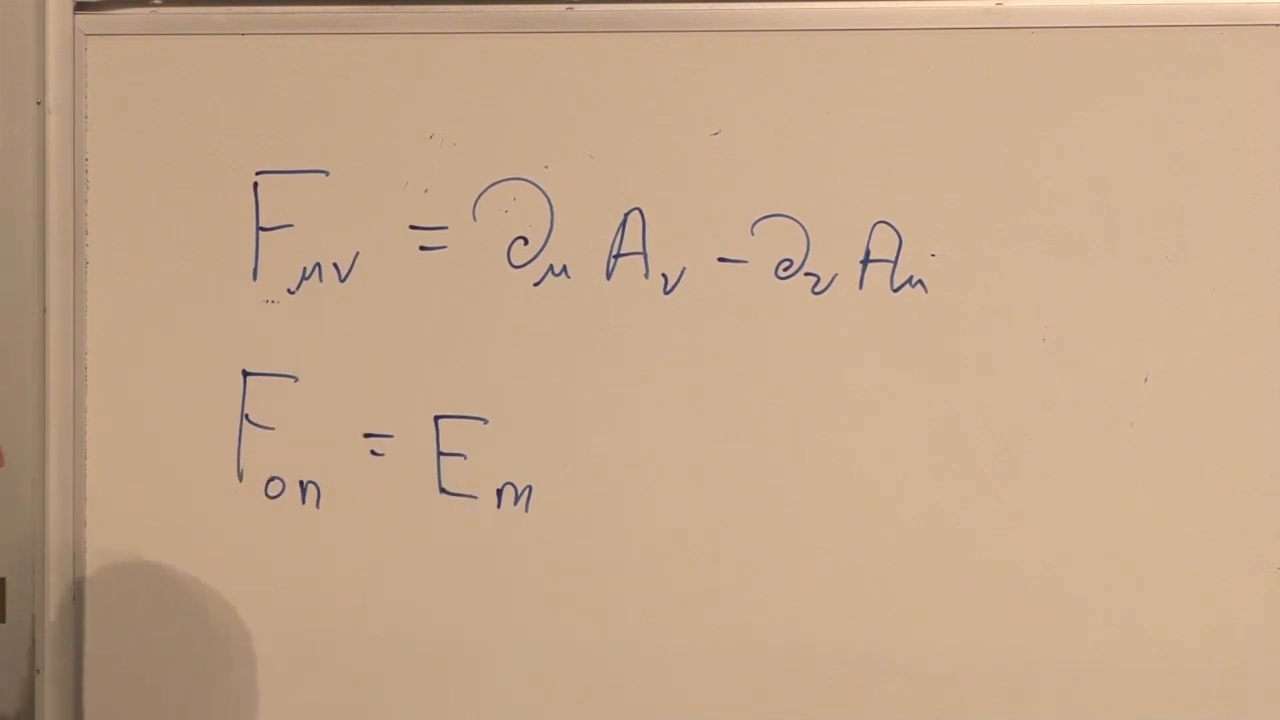
\includegraphics[width=\linewidth]{lecture_08_figure_02.png}
\caption{Определение тензора поля и смешанная временная--пространственная компонента, отождествляемая с электрическим полем.}
\par\smallskip
\textit{Кадр лекции: 00:13:15.}
\end{figure}

Магнитное соотношение представляет собой пространственную часть того же определения. Например,
\begin{equation}
B_x
=
\partial_yA_z-\partial_zA_y
=
F_{yz},
\end{equation}
а две остальные компоненты получаются циклической перестановкой.

\begin{figure}[H]
\centering
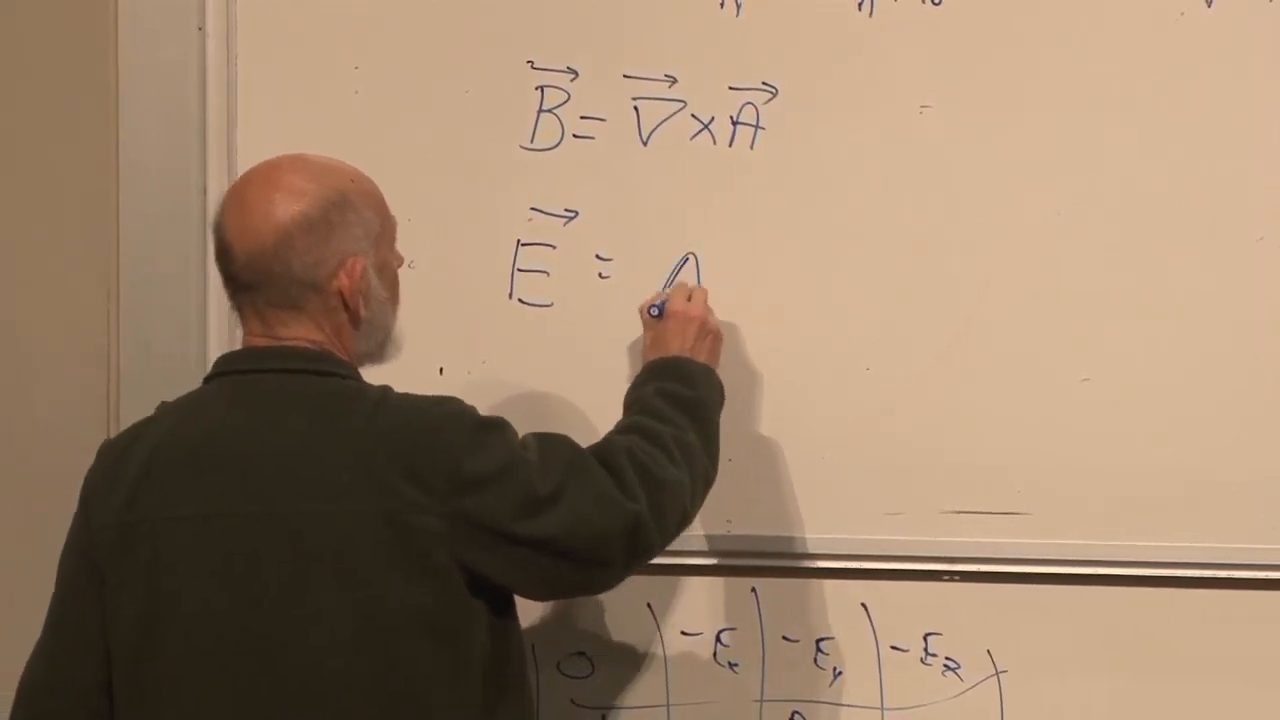
\includegraphics[width=\linewidth]{lecture_08_figure_03.png}
\caption{Формулы через векторный потенциал для электрического поля и для магнитного ротора, выписанные на доске.}
\par\smallskip
\textit{Кадр лекции: 00:14:00.}
\end{figure}

\subsection{Матрица компонент}

Пусть первый индекс тензора нумерует строки, а второй — столбцы, в порядке \(0,x,y,z\). Тогда
\begin{equation}
F_{\mu\nu}
=
\begin{pmatrix}
0&E_x&E_y&E_z\\
-E_x&0&B_z&-B_y\\
-E_y&-B_z&0&B_x\\
-E_z&B_y&-B_x&0
\end{pmatrix}.
\label{eq:f-lower-matrix}
\end{equation}
Смешанная временная--пространственная часть содержит \(\mathbf E\); пространственный блок \(3\times3\) содержит \(\mathbf B\). Нижний треугольник не несет новой информации, потому что он получается из верхнего сменой знака.

\begin{figure}[H]
\centering
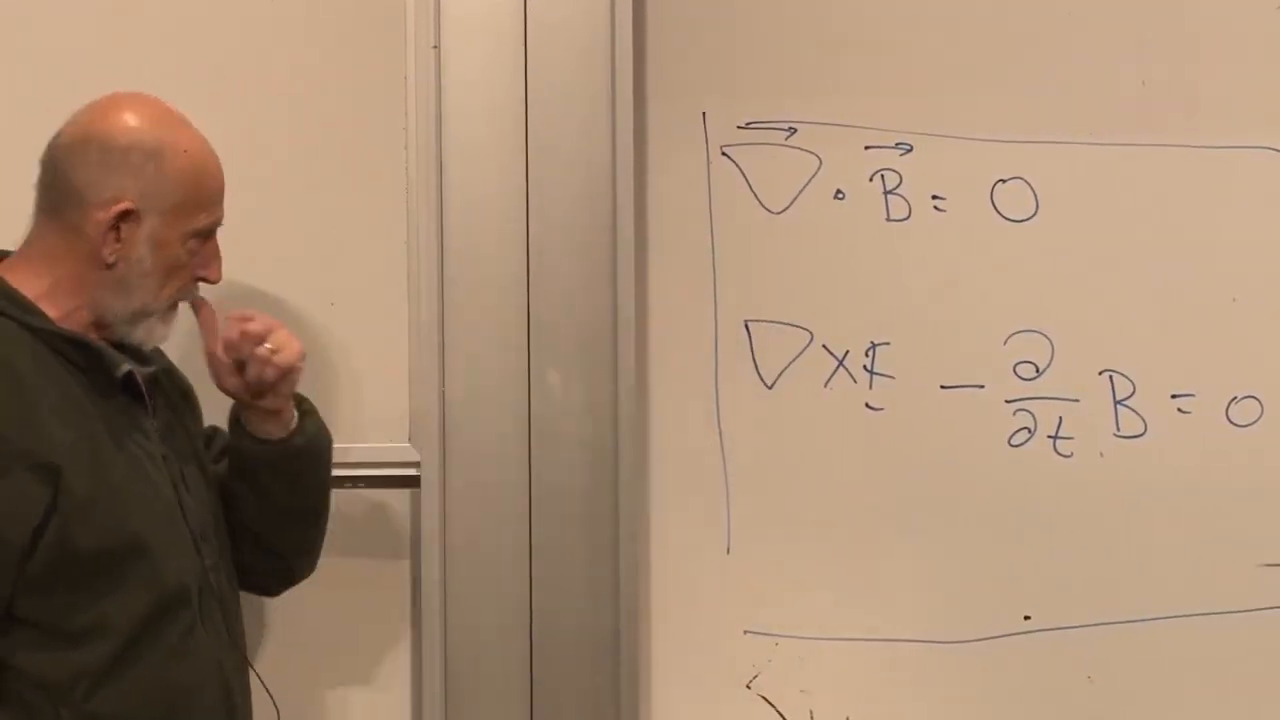
\includegraphics[width=\linewidth]{lecture_08_figure_04.png}
\caption{Полный электромагнитный тензор с нижними индексами, с электрической частью по краю и магнитным пространственным блоком.}
\par\smallskip
\textit{Кадр лекции: 00:17:15.}
\end{figure}

Поднятие обоих индексов меняет знак у каждого электрического элемента и оставляет магнитные элементы без изменения:
\begin{equation}
F^{\mu\nu}
=
\begin{pmatrix}
0&-E_x&-E_y&-E_z\\
E_x&0&B_z&-B_y\\
E_y&-B_z&0&B_x\\
E_z&B_y&-B_x&0
\end{pmatrix}.
\label{eq:f-upper-matrix}
\end{equation}
Электрическая компонента несет один временной индекс и поэтому получает один знак минус. Магнитная компонента несет два пространственных индекса и не получает ни одного.

\begin{classroomqa}
\audiencequestion{Правильно ли я читаю матрицу: у магнитных компонент нет временного индекса?}
\lecturerresponse{Да. Они занимают чисто пространственный блок. Электрические компоненты — это как раз смешанные элементы время--пространство в первой строке и первом столбце. \lecturetimestamp{00:18:55}}
\end{classroomqa}

\section{Буст чисто магнитного поля}

Рассмотрим буст вдоль \(x\) при \(c=1\):
\begin{align}
t'&=\gamma(t-vx),
&
x'&=\gamma(x-vt),
&
y'&=y,
&
z'&=z,
\end{align}
где
\begin{equation}
\gamma=\frac{1}{\sqrt{1-v^2}}.
\end{equation}
В матричной форме
\begin{equation}
x'^\mu
=
\Lambda^\mu{}_\nu x^\nu,
\qquad
\Lambda^\mu{}_\nu
=
\begin{pmatrix}
\gamma&-\gamma v&0&0\\
-\gamma v&\gamma&0&0\\
0&0&1&0\\
0&0&0&1
\end{pmatrix}.
\label{eq:x-boost}
\end{equation}

\begin{classroomqa}
\audiencequestion{Не пропущен ли знак минус в матрице буста?}
\lecturerresponse{Да. У внедиагональных элементов типа время--пространство стоят знаки минус, требуемые \(t'=\gamma(t-vx)\) и \(x'=\gamma(x-vt)\). Исправление вносится до того, как используется преобразование поля. \lecturetimestamp{00:23:50}}
\end{classroomqa}

\begin{figure}[H]
\centering
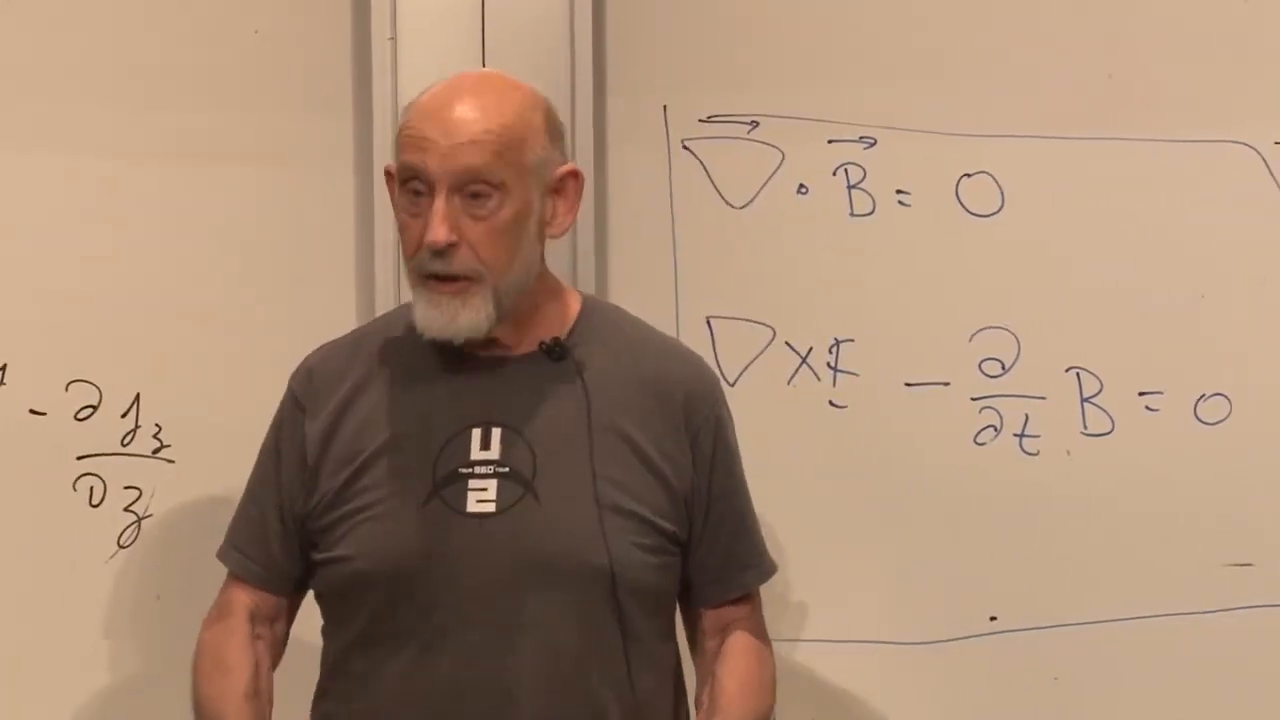
\includegraphics[width=\linewidth]{lecture_08_figure_05.png}
\caption{Исправленная матрица буста Лоренца для движения вдоль оси \(x\).}
\par\smallskip
\textit{Кадр лекции: 00:24:00.}
\end{figure}

Каждый верхний тензорный индекс преобразуется так же, как верхний векторный индекс. Поэтому
\begin{equation}
F'^{\mu\nu}
=
\Lambda^\mu{}_\sigma
\Lambda^\nu{}_\tau
F^{\sigma\tau}.
\label{eq:f-boost-law}
\end{equation}
Повторяющиеся \(\sigma\) и \(\tau\) — фиктивные индексы. Для тензора с большим числом индексов для каждого индекса появлялась бы своя матрица преобразования.

\begin{figure}[H]
\centering
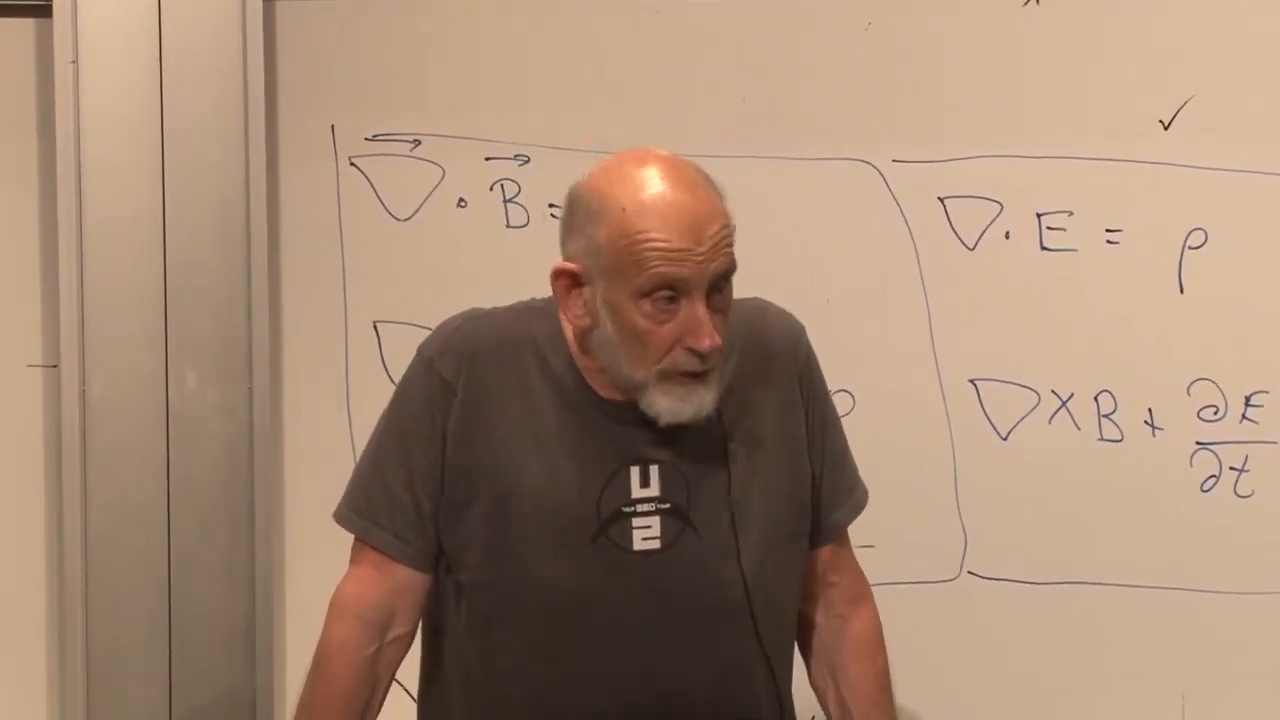
\includegraphics[width=\linewidth]{lecture_08_figure_06.png}
\caption{Закон лоренцева преобразования для тензора второго ранга, с одной матрицей буста для каждого индекса тензора поля.}
\par\smallskip
\textit{Кадр лекции: 00:26:40.}
\end{figure}

\subsection{Компонента, становящаяся электрической}

Предположим, что в нештрихованной системе отсчета имеется только магнитное поле \(B_y\). В соглашениях из уравнения~\eqref{eq:f-upper-matrix} соответствующая независимая компонента имеет вид
\begin{equation}
F^{xz}=-B_y.
\end{equation}
Ищем штрихованную смешанную компоненту \(F'^{0z}\), потому что ей соответствует \(z\)-компонента электрического поля в штрихованной системе. Из уравнения \eqref{eq:f-boost-law} получаем
\begin{align}
F'^{0z}
&=
\Lambda^0{}_\sigma
\Lambda^z{}_\tau F^{\sigma\tau}
\\
&=
\Lambda^0{}_x\Lambda^z{}_zF^{xz}
\\
&=
(-\gamma v)(1)(-B_y)
=
\gamma vB_y.
\end{align}
Поскольку в этом соглашении \(F'^{0z}=-E'_z\),
\begin{equation}
E'_z=-\gamma vB_y.
\label{eq:boosted-electric-field}
\end{equation}
Знак зависит от принятых соглашений об осях и поле; инвариантный смысл вычисления таков:
\begin{equation}
\lvert E'_z\rvert
=
\gamma\lvert vB_y\rvert
\ne0.
\end{equation}
Двойная сумма схлопывается, потому что у исходного поля есть только эта одна независимая магнитная компонента.

\begin{figure}[H]
\centering
\includegraphics[width=\linewidth]{lecture_08_figure_07.png}
\caption{Выбранная компонента тензора после буста, показывающая множитель \(\gamma v\) при исходной магнитной компоненте.}
\par\smallskip
\textit{Кадр лекции: 00:32:30.}
\end{figure}

Выберем штрихованную систему отсчета, сопутствующую заряду. Тогда заряд покоится, так что магнитной части \(q\,\mathbf v'\times\mathbf B'\) в действующей на него силе нет. Однако сила не исчезает: это \(q\mathbf E'\). Магнитная сила для лабораторного наблюдателя и электрическая сила для сопутствующего наблюдателя — два описания одного и того же события.

Это и есть ответ на загадку из первого абзаца Эйнштейна. Этому вопросу были посвящены примерно первые 40 минут этой лекции; историческая шутка состоит в том, что у Эйнштейна это заняло гораздо больше времени. Это вычисление стоит затраченного времени, потому что превращает лозунг о том, что электрическое и магнитное поля смешиваются, в одну явную компоненту тензора.

\section{Уравнения Максвелла: тождества и динамика}

Теперь перейдём от силы, действующей на заряд, к уравнениям поля. Они будут выведены из действия на следующей лекции. Здесь цель состоит в том, чтобы сначала сформулировать их, понять две их различные логические роли и записать половину, основанную на тождествах, в ковариантном виде.

\begin{classroomqa} \audiencequestion{Разве мы уже не вывели эти уравнения?} \lecturerresponse{Мы вывели уравнение движения заряженной частицы в заданном электромагнитном поле. Уравнения Максвелла — это уравнения движения для самого поля, включая отклик поля на заряд и ток. \lecturetimestamp{00:35:10}} \end{classroomqa}

\begin{classroomqa} \audiencequestion{Сколько существует уравнений Максвелла?} \lecturerresponse{Существует 8 скалярных уравнений для компонент. Векторная запись объединяет их в 2 скалярных уравнения и 2 трёхкомпонентных векторных уравнения, которые по соглашению называют четырьмя уравнениями Максвелла. \lecturetimestamp{00:35:24}} \end{classroomqa}

Мы по-прежнему используем единицы, в которых \(c=1\) и обычные вакуумные константы поглощены в определениях заряда и тока. Четыре из 8 уравнений для компонент следуют из определения \(F=dA\). Это кинематические тождества. Остальные 4 — динамические и могли бы измениться, если бы изменилось действие поля.

\subsection{Три элементарные векторные операции}

Для дифференцируемого трёхвекторного поля \(\mathbf A\), \begin{align}
(\boldsymbol\nabla\times\mathbf A)_x
&=
\partial_yA_z-\partial_zA_y,
\\
\boldsymbol\nabla\cdot\mathbf A
&=
\partial_xA_x+\partial_yA_y+\partial_zA_z.
\end{align} Остальные компоненты ротора получаются циклической перестановкой \(x\to y\to z\to x\). Для скалярного поля \(s\), \begin{equation}
\boldsymbol\nabla s
=
(\partial_xs,\partial_ys,\partial_zs).
\end{equation} Таким образом, ротор — это вектор, дивергенция — скаляр, а градиент — вектор.

\begin{classroomqa} \audiencequestion{Нужно ли кому-нибудь полностью повторить определения ротора и дивергенции?} \lecturerresponse{Определения через компоненты записаны, но нет необходимости расписывать все остальные компоненты. Они получаются циклической перестановкой координатных меток. \lecturetimestamp{00:37:32}} \end{classroomqa}

Из коммутативности частных производных для гладких функций следуют два тождества: \begin{align}
\boldsymbol\nabla\cdot
(\boldsymbol\nabla\times\mathbf A)
&=0,
\label{eq:div-curl}
\\
\boldsymbol\nabla\times
(\boldsymbol\nabla s)
&=\mathbf0.
\label{eq:curl-grad}
\end{align}

\begin{classroomqa} \audiencequestion{Следует ли нам полностью выписать покомпонентное доказательство того, что дивергенция ротора равна нулю?} \lecturerresponse{Аудитория отказывается. При раскрытии компонент возникают пары вида \(\partial_x\partial_yA_z\) и \(-\partial_y\partial_xA_z\), которые сокращаются, поскольку порядок дифференцирования можно переставлять. \lecturetimestamp{00:40:13}} \end{classroomqa}

\begin{figure}[H] \centering
\includegraphics[width=\linewidth]{lecture_08_figure_08.png} \caption{Тождества о дивергенции ротора и роторе градиента, использованные при выводе половины уравнений Максвелла.} \par\smallskip
\textit{Кадр лекции: 00:41:40.} \end{figure}

\subsection{Отсутствие магнитного источника при задании через векторный потенциал}

Взятие дивергенции от уравнения~\eqref{eq:b-from-a} даёт \begin{equation}
\boldsymbol\nabla\cdot\mathbf B
=
\boldsymbol\nabla\cdot
(\boldsymbol\nabla\times\mathbf A)
=0.
\label{eq:div-b-zero}
\end{equation} Никакое уравнение движения не использовалось. Результат следует только из описания через потенциал и гладкости производных.

\begin{figure}[H] \centering
\includegraphics[width=\linewidth]{lecture_08_figure_09.png} \caption{Дивергенция магнитного поля сведена к дивергенции ротора.} \par\smallskip
\textit{Кадр лекции: 00:43:05.} \end{figure}

\begin{classroomqa} \audiencequestion{Чему равна дивергенция электрического поля?} \lecturerresponse{В используемых единицах она равна плотности электрического заряда, \(\boldsymbol\nabla\cdot\mathbf E=\rho\). Точечный заряд — это наглядный пример источника, от которого расходятся линии электрического поля. \lecturetimestamp{00:43:20}} \end{classroomqa}

На этом элементарном уровне уравнение~\eqref{eq:div-b-zero} говорит, что плотность магнитного заряда равна нулю. Гладкий, глобально определённый векторный потенциал не может породить магнитно-монопольный источник. Позже это утверждение придётся уточнить: монополи можно описывать потенциалами, определёнными на перекрывающихся областях, или сингулярными выборами калибровки. Лекция откладывает это уточнение.

\subsection{Уравнение Фарадея из электрического потенциала}

Уравнение~\eqref{eq:e-from-a} в трёхвекторной записи имеет вид \begin{equation}
\mathbf E
=
\frac{\partial\mathbf A}{\partial t}
-\boldsymbol\nabla A_0.
\label{eq:e-vector-potential}
\end{equation} Хотя \(A_0\) входит в четырёхвектор, при обычных пространственных поворотах это скаляр. Возьмём ротор: \begin{align}
\boldsymbol\nabla\times\mathbf E
&=
\boldsymbol\nabla\times
\frac{\partial\mathbf A}{\partial t}
-
\boldsymbol\nabla\times
(\boldsymbol\nabla A_0)
\\
&=
\frac{\partial}{\partial t}
(\boldsymbol\nabla\times\mathbf A)
\\
&=
\frac{\partial\mathbf B}{\partial t}.
\end{align} Пространственный ротор коммутирует с производной по времени, тогда как ротор градиента равен нулю.

\begin{figure}[H] \centering
\includegraphics[width=\linewidth]{lecture_08_figure_10.png} \caption{Ротор магнитного поля, формула для электрического потенциала и начало вычисления ротора в одном завершённом состоянии доски.} \par\smallskip
\textit{Кадр лекции: 00:47:45.} \end{figure}

Следовательно, четыре однородных уравнения для компонент имеют вид \begin{align}
\boldsymbol\nabla\cdot\mathbf B&=0,
\label{eq:homogeneous-div}
\\
\boldsymbol\nabla\times\mathbf E
-\frac{\partial\mathbf B}{\partial t}
&=\mathbf0.
\label{eq:homogeneous-curl}
\end{align} Первое — одно скалярное уравнение; второе — одно трёхкомпонентное векторное уравнение.

\begin{figure}[H] \centering
\includegraphics[width=\linewidth]{lecture_08_figure_11.png} \caption{Пара уравнений Максвелла без источников, полученная непосредственно из определений потенциала.} \par\smallskip
\textit{Кадр лекции: 00:48:45.} \end{figure}

\subsection{Динамическая половина}

Оставшиеся уравнения имеют вид \begin{align}
\boldsymbol\nabla\cdot\mathbf E&=\rho,
\label{eq:gauss-electric}
\\
\boldsymbol\nabla\times\mathbf B
+\frac{\partial\mathbf E}{\partial t}
&=-\mathbf J.
\label{eq:ampere-maxwell}
\end{align} Они не являются следствиями \(F=dA\). Они описывают, как источники создают и изменяют поле, и на следующей лекции будут выведены из электромагнитного действия. Знак минус при токе фиксирован уже выбранными соглашениями: \(F_{0i}=E_i\), \(F_{ij}=\epsilon_{ijk}B_k\) и \(\partial_\mu F^{\mu\nu}=J^\nu\). На доске по ходу лекции сперва ставят \(\mathbf J\) справа без этого минуса; возникающее несоответствие с сохранением заряда замечают и исправляют на следующей лекции.

\begin{classroomqa} \audiencequestion{Какого рода величина стоит в правой части уравнения с ротором?} \lecturerresponse{Левая часть — трёхвектор, поэтому правая часть — тоже трёхвектор, называемый плотностью электрического тока \(\mathbf J\). Правая часть уравнения Гаусса — трёхмерная скалярная плотность заряда \(\rho\). \lecturetimestamp{00:50:36}} \end{classroomqa}

\begin{figure}[H] \centering
\includegraphics[width=\linewidth]{lecture_08_figure_12.png} \caption{Четыре уравнения Максвелла, сгруппированные в пару, основанную на тождествах, и динамическую пару с источниками.} \par\smallskip
\textit{Кадр лекции: 00:50:40.} \end{figure}

\section{Заряд и ток как поток в пространстве-времени}

Теперь символам \(\rho\) и \(\mathbf J\) нужно придать геометрический смысл. Плотность заряда — это заряд на единицу объёма; плотность тока — это заряд, пересекающий ориентированную площадку за единицу времени. Лекция выводит обе величины из мировых линий, чтобы их последующее объединение в четырёхвектор не выглядело случайным.

\subsection{Отступление, вызванное соседней доской}

Прежде чем рисовать эти мировые линии, уравнения, видимые в соседней комнате, вызывают краткое педагогическое отступление. На одном из предстоящих курсов предполагалось знакомить преподавателей-математиков с квантовой механикой; им была нужна подготовка, необходимая для квантовой теории поля и её связей с современной математикой. Трудность возникает в обе стороны: физик должен сделать явными неявные физические привычки, а математик должен понять, что именно формальные структуры должны описывать.

\begin{classroomqa} \audiencequestion{Кому, как ожидается, эта преподавательская задача покажется тягостной?} \lecturerresponse{Возможно, обеим сторонам: физикам, преподающим непривычной аудитории, и математикам, сталкивающимся с физическими привычками, стоящими за формализмом. Тем не менее ожидается, что это будет увлекательно. Затем лекция возвращается к заряду и току. \lecturetimestamp{00:53:20}} \end{classroomqa}

\subsection{Плотность заряда}

Изобразим время по вертикали и будем считать, что остальные изображённые направления представляют трёхмерное пространство. Заряженные частицы прочерчивают мировые линии. В один фиксированный момент времени поместим небольшой пространственный куб объёма \(\Delta V\) поперёк этого пучка мировых линий и просуммируем заряды частиц внутри него. Плотность заряда равна \begin{equation}
\rho(t,\mathbf x)
=
\lim_{\Delta V\to0}
\frac{\Delta Q}{\Delta V}.
\label{eq:charge-density}
\end{equation} Двумерный квадрат на доске изображает трёхмерный куб; недостающее пространственное направление опущено только потому, что 4 измерения невозможно нарисовать на плоской доске.

\begin{figure}[H] \centering
\includegraphics[width=\linewidth]{lecture_08_figure_13.png} \caption{Мировые линии заряженных частиц, пересекающие малую пространственную ячейку, с \(\rho=\Delta Q/\Delta V\).} \par\smallskip
\textit{Кадр лекции: 00:57:20.} \end{figure}

\subsection{Плотность тока}

Повернём пространственно-временную ячейку набок. Чтобы определить \(J_x\), выберем маленькое окно площади \(\Delta A_x\) в плоскости \(yz\), перпендикулярное оси \(x\). Подсчитаем суммарный заряд, проходящий со стороны с отрицательным \(x\) на сторону с положительным \(x\) за \(\Delta t\): \begin{equation}
J_x
=
\lim_{\Delta A_x,\Delta t\to0}
\frac{\Delta Q_x}{\Delta A_x\,\Delta t}.
\label{eq:jx-window}
\end{equation} Ориентация задаёт знак. Окна, перпендикулярные \(y\) и \(z\), таким же образом определяют \(J_y\) и \(J_z\).

Рисунок на доске честно показывает трудность: окно в плоскости \(yz\) выглядит скорее как окно в потолке, чем как окно в стене. Просто существенных осей больше, чем можно одновременно показать. Инвариантное определение однозначно, даже когда эскиз — нет.

\begin{classroomqa}
\audiencequestion{Окно на рисунке находится на потолке?}
\lecturerresponse{В аналогии с комнатой — да. Важно то, что его плоскость перпендикулярна направлению \(x\). Площадь \(yz\) измеряет ток, направленный вдоль \(x\) и пересекающий её. \lecturetimestamp{00:59:38}}
\end{classroomqa}

\begin{figure}[H]
\centering
\includegraphics[width=\linewidth]{lecture_08_figure_14.png}
\caption{Ток заряда через поперечное окно, где \(J_x=\Delta Q/(\Delta A\,\Delta t)\).}
\par\smallskip
\textit{Кадр лекции: 01:01:40.}
\end{figure}

\begin{figure}[H]
\centering
\includegraphics[width=\linewidth]{lecture_08_figure_15.png}
\caption{Три компоненты тока, определённые через заряд, пересекающий окна, нормальные к трём пространственным осям.}
\par\smallskip
\textit{Кадр лекции: 01:02:40.}
\end{figure}

Все 4 величины определяются по одной схеме. Пространственный объём в фиксированный момент времени — это гиперповерхность, перпендикулярная оси времени, так что \(\rho\) есть поток заряда через окно, перпендикулярное оси времени. Величины \(J_i\) — это потоки через окна, перпендикулярные пространственным направлениям.

\begin{classroomqa}
\audiencequestion{Эти 4 числа — один поток во временном направлении и 3 потока в пространственных направлениях?}
\lecturerresponse{Это как раз и есть полезная картина. Пространственный объём — окно, перпендикулярное оси времени; 3 поперечные площади — окна, перпендикулярные \(x\), \(y\) и \(z\). Эти 4 потока нужно рассматривать вместе. \lecturetimestamp{01:04:14}}
\end{classroomqa}

Это подсказывает контравариантный четырёхток
\begin{equation}
J^\mu
=
(\rho,J_x,J_y,J_z).
\label{eq:four-current}
\end{equation}

\begin{classroomqa}
\audiencequestion{Где входит метрика, и этот ток ковариантный или контравариантный?}
\lecturerresponse{В том виде, как он определён здесь, \(\rho\) и 3 \(J_i\) образуют компоненты \(J^\mu\), четырёхвектора с верхним индексом, то есть контравариантного. Метрика опускает индекс, когда требуется \(J_\mu\). Ковариантная формулировка уравнений Максвелла покажет, почему выбор верхнего индекса естествен.
\lecturetimestamp{01:04:48}}
\end{classroomqa}

\section{Интерлюдия в перерыве: сигналы вблизи чёрной дыры}

Во время запланированного перерыва вопросы возвращаются к предыдущему обсуждению чёрных дыр. Хотя это отступление от электродинамики, обмен репликами в аудитории получается содержательным и иллюстрирует ту же дисциплину: нужно разделять описания, данные разными наблюдателями.

\begin{classroomqa}
\audiencequestion{Если удалённый наблюдатель видит, что падающий внутрь объект замедляется вблизи горизонта, не должна ли чёрная дыра выглядеть покрытой всем, что когда-либо в неё упало?}
\lecturerresponse{В координатном времени Шварцшильда классическое падение выглядит как асимптотическое приближение к горизонту. Можно представлять себе последовательные порции вещества как всё более сжатые слои у горизонта. Однако в операционном смысле исходящий сигнал всё сильнее запаздывает, испытывает всё больший красный сдвиг и слабеет. Свет, испущенный с обычной локальной частотой, приходит сначала как оптический, затем как инфракрасный, микроволновый и радиосигнал, причём каждый фотон несёт всё меньшую энергию. Ни один реалистичный удалённый детектор не будет вечно видеть яркий застывший объект; он угасает в черноту.
\lecturetimestamp{01:06:11}}
\end{classroomqa}

Часы падающего наблюдателя и испускаемый локально свет фонарика остаются для него обычными. Описание издали отличается, потому что частота и темп прихода сигнала смещены в красную сторону. При конечной энергии и конечной полосе пропускания фактически существует последняя различимая часть сообщения.

\begin{classroomqa}
\audiencequestion{Объект асимптотически приближается к горизонту событий?}
\lecturerresponse{Таково удалённое описание в координатах Шварцшильда. В квантовомеханическом отношении затухающий сигнал нужно также отличать от излучения Хокинга самой чёрной дыры. На достаточно поздних временах слабый, испытавший красное смещение сигнал наблюдательно теряется на фоне собственного излучения дыры. \lecturetimestamp{01:09:24}}
\end{classroomqa}

\begin{classroomqa}
\audiencequestion{Что если длина волны после красного смещения вырастет больше масштаба наблюдаемой Вселенной?}
\lecturerresponse{Практически сигнал теряется задолго до этого предела. На лекции даётся хокинговская картина по порядку величины: примерно один типичный квант за время светового пересечения,
\[
t_{\rm cross}\sim\frac{R_s}{c}.
\]
Для большой дыры это чрезвычайно слабое излучение, и достаточно сильно покрасневший сигнал от падающего объекта становится необнаружимым гораздо раньше любого космологического ограничения на длину волны. \lecturetimestamp{01:09:50}}
\end{classroomqa}

\begin{classroomqa}
\audiencequestion{Остаётся ли темп порядка одного кванта за время пересечения постоянным на протяжении всей жизни чёрной дыры?}
\lecturerresponse{Нет. Испаряющаяся шварцшильдовская чёрная дыра сжимается, так что её время пересечения уменьшается, а температура Хокинга растёт. Поэтому излучение ускоряется. Оценка по размерности через мгновенный радиус остаётся полезной, но радиус не постоянен. Соответственно, типичная хокинговская длина волны укорачивается по мере испарения. \lecturetimestamp{01:11:42}}
\end{classroomqa}

После перерыва, сняв пиджак, мы возвращаемся к \(\rho\) и \(\mathbf J\).

\section{Локальное сохранение заряда}

Заманчиво сформулировать сохранение заряда только так:
\begin{equation}
\frac{dQ_{\rm universe}}{dt}=0.
\end{equation}
Но этого утверждения недостаточно. Заряд мог бы исчезнуть из лаборатории и мгновенно появиться у Альфы Центавра или ещё дальше, в скоплении Кома, не изменяя полного количества. Такой закон мало что значил бы экспериментально.

Более сильное утверждение локально: заряд внутри области может меняться только за счёт пересечения границы этой области. Поместим вокруг точки маленький ящик. Если заряд в нём увеличивается, через его 6 граней должен идти суммарный ток внутрь; если уменьшается, должен идти суммарный ток наружу.

\subsection{Поток через противоположные грани}

Рассмотрим 2 грани, перпендикулярные \(x\). Входящий вклад на одной грани вычисляется при одном значении \(x\); вклад на противоположной грани вычисляется на малом расстоянии от него. Их разность, делённая на ширину ящика, стремится к
\begin{equation}
-\partial_xJ_x.
\end{equation}
Минус возникает потому, что положительный \(J_x\) определён как поток в сторону возрастания \(x\), тогда как поток наружу уменьшает заряд в ящике. Пары граней, перпендикулярных \(y\) и \(z\), аналогично дают
\(-\partial_yJ_y\) и \(-\partial_zJ_z\). Следовательно,
\begin{equation}
\frac{\partial\rho}{\partial t}
=
-\partial_xJ_x-\partial_yJ_y-\partial_zJ_z
=
-\boldsymbol\nabla\cdot\mathbf J.
\end{equation}
Эквивалентно,
\begin{equation}
\boxed{
\frac{\partial\rho}{\partial t}
+\boldsymbol\nabla\cdot\mathbf J=0
}.
\label{eq:continuity}
\end{equation}

\begin{figure}[H]
\centering
\includegraphics[width=\linewidth]{lecture_08_figure_16.png}
\caption{Локальный закон баланса
\(\dot\rho=-\boldsymbol\nabla\cdot\mathbf J\), вместе с маленьким ящиком, из граничных токов которого он следует.}
\par\smallskip
\textit{Кадр лекции: 01:20:45.}
\end{figure}

Это обычно называют уравнением непрерывности. В лекции предпочитают название \emph{локальное сохранение}: слово непрерывность может наводить на мысль о математическом предположении гладкости, тогда как физический смысл состоит в том, что заряд не может исчезнуть здесь и появиться там без тока между ними.

\subsection{Почему Максвеллу понадобился ток смещения}

Уравнение~\eqref{eq:continuity} не является независимым добавлением к уравнениям Максвелла. Возьмём производную по времени от закона Гаусса и дивергенцию закона Ампера--Максвелла:
\begin{align}
\frac{\partial\rho}{\partial t}
&=
\boldsymbol\nabla\cdot
\frac{\partial\mathbf E}{\partial t},
\\
-\boldsymbol\nabla\cdot\mathbf J
&=
\boldsymbol\nabla\cdot
(\boldsymbol\nabla\times\mathbf B)
+
\boldsymbol\nabla\cdot
\frac{\partial\mathbf E}{\partial t}
\\
&=
\boldsymbol\nabla\cdot
\frac{\partial\mathbf E}{\partial t}.
\end{align}
Тем самым левые части этих двух равенств совпадают, и получается
\(\partial_t\rho=-\boldsymbol\nabla\cdot\mathbf J\), то есть в точности
Уравнение~\eqref{eq:continuity}. Структурно существенно то, что производная по времени от \(\mathbf E\), то есть член тока смещения, необходима, чтобы соотношение для дивергенции было совместимо с сохранением заряда.

\begin{classroomqa}
\audiencequestion{Мы ведь не показали, откуда берутся 2 уравнения Максвелла с источниками, не так ли?}
\lecturerresponse{Нет. Именно их мы и будем в следующий раз выводить из действия как динамические уравнения. Закон ротора в магнитостатике был известен до Максвелла; его решающим зависящим от времени дополнением был ток смещения. Его наличие делает уравнение поля совместимым с локальным сохранением заряда. \lecturetimestamp{01:23:15}}
\end{classroomqa}

Подробное вычисление дивергенции оставлено в лекции как упражнение, но его вывод не факультативен: уравнения Максвелла требуют сохранения заряда.

\section{Четырёхток и его дивергенция}

Запишем уравнение~\eqref{eq:continuity} по компонентам:
\begin{equation}
\frac{\partial\rho}{\partial t}
+
\frac{\partial J_x}{\partial x}
+
\frac{\partial J_y}{\partial y}
+
\frac{\partial J_z}{\partial z}
=0.
\label{eq:continuity-components}
\end{equation}

\begin{figure}[H]
\centering
\includegraphics[width=\linewidth]{lecture_08_figure_17.png}
\caption{Локальное сохранение заряда, развернутое в одну производную по времени и 3 пространственные производные.}
\par\smallskip
\textit{Кадр лекции: 01:25:40.}
\end{figure}

Если \(J^\mu\) определён уравнением~\eqref{eq:four-current}, то все 4 члена образуют одну свёртку:
\begin{equation}
\boxed{\partial_\mu J^\mu=0}.
\label{eq:four-current-conservation}
\end{equation}
Нижний индекс у \(\partial_\mu\) свёртывается с верхним индексом у \(J^\mu\), поэтому результат является скаляром Лоренца. Геометрическая конструкция с окнами уже подсказывала этот закон преобразования: \(\rho\) и 3 компоненты тока — это 4 ориентации одного и того же потока заряда.

\begin{figure}[H]
\centering
\includegraphics[width=\linewidth]{lecture_08_figure_18.png}
\caption{Компоненты \((\rho,J_x,J_y,J_z)\), собранные в \(J^\mu\) и свёрнутые с четырёхградиентом.}
\par\smallskip
\textit{Кадр лекции: 01:27:10.}
\end{figure}

\begin{classroomqa}
\audiencequestion{Когда временная производная \(\rho\) стала частной производной?}
\lecturerresponse{С самого начала это была частная производная. Мы держим пространственный объём фиксированным и спрашиваем, как меняется его плотность заряда при изменении времени. Мы не прослеживаем движущуюся траекторию, так что \(\dot\rho\) здесь означает
\(\partial\rho/\partial t\) при фиксированных \(x,y,z\).
\lecturetimestamp{01:28:20}}
\end{classroomqa}

\section{Однородные уравнения в ковариантной форме}

Теперь у нас есть необходимые объекты:
\begin{itemize}
\item \(\mathbf E\) и \(\mathbf B\) — шесть независимых компонент антисимметричного тензора \(F_{\mu\nu}\);
\item \(\rho\) и \(\mathbf J\) — четыре компоненты \(J^\mu\);
\item локальный закон сохранения задаётся скалярным уравнением
\(\partial_\mu J^\mu=0\).
\end{itemize}

Остающаяся задача этой лекции — записать однородную пару уравнений Максвелла, уравнения~\eqref{eq:homogeneous-div} и
\eqref{eq:homogeneous-curl}, в виде одного тензорного уравнения.

\subsection{Циклическая производная}

Ответ таков:
\begin{equation}
\boxed{
\partial_\sigma F_{\nu\tau}
+
\partial_\nu F_{\tau\sigma}
+
\partial_\tau F_{\sigma\nu}
=0
}.
\label{eq:bianchi}
\end{equation}
Три члена циклически распределяют индекс производной и два индекса тензора поля. Это часто сокращённо записывают как
\begin{equation}
\partial_{[\sigma}F_{\nu\tau]}=0,
\end{equation}
где скобки обозначают антисимметризацию.

\begin{figure}[H]
\centering
\includegraphics[width=\linewidth]{lecture_08_figure_19.png}
\caption{Циклическое трёхиндексное уравнение, объединяющее однородные уравнения Максвелла.}
\par\smallskip
\textit{Кадр лекции: 01:33:20.}
\end{figure}

\subsection{Все три индекса пространственные}

Положим
\begin{equation}
(\sigma,\nu,\tau)=(x,y,z).
\end{equation}
Тогда
\begin{align}
0
&=
\partial_xF_{yz}
+
\partial_yF_{zx}
+
\partial_zF_{xy}
\\
&=
\partial_xB_x+\partial_yB_y+\partial_zB_z
\\
&=
\boldsymbol\nabla\cdot\mathbf B.
\end{align}
Следовательно, чисто пространственная компонента
уравнения~\eqref{eq:bianchi} есть в точности условие отсутствия магнитной
дивергенции.

\begin{figure}[H]
\centering
\includegraphics[width=\linewidth]{lecture_08_figure_20.png}
\caption{Чисто пространственная компонента циклического тождества сводится к
\(\partial_xB_x+\partial_yB_y+\partial_zB_z=0\).}
\par\smallskip
\textit{Кадр лекции: 01:35:30.}
\end{figure}

\subsection{Один временной индекс}

Выберем, например,
\begin{equation}
(\sigma,\nu,\tau)=(y,x,0).
\end{equation}
Тогда уравнение~\eqref{eq:bianchi} объединяет две пространственные производные от
электрических компонент с производной по времени от магнитной компоненты:
\begin{equation}
\partial_yF_{x0}
+
\partial_xF_{0y}
+
\partial_0F_{yx}
=0.
\end{equation}
Используя матрицу из уравнения~\eqref{eq:f-lower-matrix}, это даёт одну
компоненту
\begin{equation}
\boldsymbol\nabla\times\mathbf E
-\frac{\partial\mathbf B}{\partial t}
=\mathbf0,
\end{equation}
причём относительные знаки фиксируются антисимметрией. Выбор других пар
пространственных индексов даёт две остальные компоненты ротора.

\begin{figure}[H]
\centering
\includegraphics[width=\linewidth]{lecture_08_figure_21.png}
\caption{Проверка компоненты с одним временным и двумя пространственными индексами, дающая одну компоненту
уравнения Фарадея.}
\par\smallskip
\textit{Кадр лекции: 01:38:20.}
\end{figure}

Есть и прямое доказательство. Подставьте
уравнение~\eqref{eq:field-tensor-definition} в
уравнение~\eqref{eq:bianchi}. Возникают шесть членов со вторыми производными, и они
попарно сокращаются, поскольку частные производные коммутируют. Это
четырёхмерная версия тождеств о дивергенции ротора и роторе градиента.

\begin{classroomqa}
\audiencequestion{Есть ли в имени Bianchi буква \(h\)?}
\lecturerresponse{Да. Циклическое уравнение — это электромагнитное
тождество Бьянки, частный случай геометрического тождества, которое также встречается
в общей теории относительности. Его более глубокая геометрическая интерпретация
откладывается.
\lecturetimestamp{01:40:28}}
\end{classroomqa}

\subsection{Почему 64 записанные компоненты содержат только 4 уравнения}

Кажется, что три индекса, каждый из которых может принимать
4 значения, дают
\(4^3=64\) уравнения. Антисимметрия устраняет избыточность:
\begin{itemize}
\item если любые два индекса совпадают, циклическое выражение тождественно
обращается в нуль;
\item если все три индекса различны, перестановки воспроизводят одно и то же
уравнение с точностью до знака;
\item в четырёх измерениях существует только
\(\binom{4}{3}=4\) неупорядоченных троек различных индексов.
\end{itemize}
Существует \(24\) упорядоченных троек, в которых все индексы различны; они распадаются на
четыре набора по шесть перестановок. Оставшиеся \(40\) упорядоченных троек
обращаются в нуль. Четыре независимых уравнения — это одно уравнение об отсутствии магнитной
дивергенции и три компоненты уравнения Фарадея.

\begin{classroomqa}
\audiencequestion{У тензора поля шесть независимых компонент, но
трёхиндексное выражение, по-видимому, содержит 64 уравнения. Почему остаются только
4?}
\lecturerresponse{Повторяющиеся индексы дают нуль, а перестановки трёх
различных индексов повторяют одно и то же соотношение с точностью до знака. Поэтому кажущиеся
64 компоненты сводятся к 4 независимым уравнениям.
\lecturetimestamp{01:41:58}}
\end{classroomqa}

Уравнение~\eqref{eq:bianchi} явно тензорно и потому
лоренц-ковариантно. В гладком описании с одним потенциалом оно также утверждает,
что нет ни плотности магнитного заряда, ни магнитного тока. Динамическая
пара с источниками остаётся ровно на той границе, до которой дошла
лекция: её ковариантное уравнение и вывод из действия относятся к следующему
занятию.

\section{Дуальность и вопрос о монополе}

В заключительных вопросах мы возвращаемся к кажущейся асимметрии между электрическими и
магнитными источниками. В пустом пространстве уравнения Максвелла допускают
поворот электрической--магнитной дуальности
\begin{equation}
\mathbf E\longrightarrow\mathbf B,
\qquad
\mathbf B\longrightarrow-\mathbf E.
\label{eq:duality-quarter-turn}
\end{equation}
Это поворот на 90 градусов в абстрактной плоскости с осями
\(\mathbf E\) и \(\mathbf B\), а не отражение, которое лишь меняет местами
их обозначения. При наличии одновременно электрических и магнитных источников
электрический и магнитный четырёхтоки должны поворачиваться одновременно.

\begin{figure}[H]
\centering
\includegraphics[width=\linewidth]{lecture_08_figure_22.png}
\caption{Заключительная иллюстрация электрической--магнитной дуальности: поворот на четверть оборота в
плоскости \(E\)-\(B\), а не простая перестановка.}
\par\smallskip
\textit{Кадр лекции: 01:45:00.}
\end{figure}

\begin{classroomqa}
\audiencequestion{Если уравнения без источников дуальны при взаимной
замене электрического и магнитного, почему тогда электрические компоненты являются компонентами время--пространство,
тогда как магнитные компоненты являются компонентами пространство--пространство?}
\lecturerresponse{Это различие в
\(F_{\mu\nu}\) зависит от системы отсчёта, а уравнения без источников допускают дуальное вращение.
Правильная операция —
\(\mathbf E\to\mathbf B\) и
\(\mathbf B\to-\mathbf E\), причём токи источников поворачиваются аналогично, если
включить магнитный заряд. При прямой перестановке теряется требуемый
знак. \lecturetimestamp{01:43:25}}
\end{classroomqa}

\begin{classroomqa}
\audiencequestion{Не делает ли чистая тензорная картина магнитный монополь
бессмысленным?}
\lecturerresponse{Нет. Это означает, что монополь нельзя представить
одним гладким векторным потенциалом во всём пространстве. Вместо этого
потенциал должен либо задаваться по кускам, либо становиться сингулярным калибровочно-зависимым образом, либо заменяться
эквивалентным дуальным описанием. Элементарный магнитный монополь не наблюдался,
и в лекции обещано вернуться к тому, как монополи вписываются в
формализм, вместо того чтобы форсировать этот вопрос в конце вечера.
\lecturetimestamp{01:45:50}}
\end{classroomqa}

Поэтому лекция заканчивается на точно обозначенной границе. Теория относительности объяснила
, почему электрическое и магнитное поля смешиваются. Определения через потенциалы дали
однородные уравнения Максвелла и их форму Бьянки. Поток заряда стал
четырёхтоком, а локальный закон сохранения стал
\(\partial_\mu J^\mu=0\). Остаётся динамическая часть: электромагнитное
действие и ковариантное уравнение поля с источником.
